
%% bare_conf.tex V1.3 2007/01/11 by Michael Shell See: http://www.michaelshell.org/
%znak procenta pretvara ostatak reda u komentar
\documentclass[conference]{IEEEtran}
%odredjujemo tip dokumenta, kao sto je book, article, report
% razliciti tipovi dokumenata podrazumevaju razlicite komande, 
%pa se moze desiti da ono sto je radilo u jednom, ne radi u drugom
%
%
\usepackage[utf8]{inputenc}%za posebne karaktere npr u imenima, bez toga nema čćžš%
\usepackage[T1]{fontenc} %za slovo Đ zaboga, mora posebno%
\usepackage{lipsum} %za lorem ipsum nasumicni tekst%
\PassOptionsToPackage{hyphens}{url} %da upakuje dugacak url u kolonu%
\usepackage[hidelinks]{hyperref}
%gornji paket će učiniti klikabilnim url adrese, kao i citate i reference ka slikama i tabelama
%\usepackage[colorlinks=true,linkcolor=blue,breaklinks]{hyperref} %za prikazivanje url adresa plavom bojom%
%\hypersetup{colorlinks=true,linkcolor=black,urlcolor=blue} %uredjivanje izgleda url na osnovu hyperref paketa%
%\urlstyle{rm}
%odkomentujte gornje tri linije ako želite hiperlinkovanje url-ova
%naredne komande menjaju neke makroe u srpski jezik. 
%Ovo je "seljačka" varijanta :) kada nećemo da se bakćemo sa babel paketima za svaki jezik
\renewcommand{\figurename}{Slika} 
\renewcommand{\tablename}{Tabela}
\renewcommand{\abstractname}{Abstrakt}
\renewcommand{\IEEEkeywordsname}{Ključne reči}
\renewcommand{\appendixname}{Prilog}
%
%
%
% Some very useful LaTeX packages include:
% (uncomment the ones you want to load)
% *** MISC UTILITY PACKAGES ***
% *** CITATION PACKAGES ***
%
\usepackage{cite} %obavezno da biste mogli da ubacujete citate, pomoću dodatnog .bib fajla
% *** GRAPHICS RELATED PACKAGES ***
%
\ifCLASSINFOpdf
   \usepackage[pdftex]{graphicx} %neophodan paket da biste mogli da prikazujete slike i grafike
  % declare the path(s) where your graphic files are
  % \graphicspath{{../pdf/}{../jpeg/}}
  % and their extensions so you won't have to specify these with
  % every instance of \includegraphics
   \DeclareGraphicsExtensions{.pdf,.jpeg,.png}
\else
  % or other class option (dvipsone, dvipdf, if not using dvips). graphicx
  % will default to the driver specified in the system graphics.cfg if no
  % driver is specified.
   \usepackage[dvips]{graphicx}
  % declare the path(s) where your graphic files are
  % \graphicspath{{../eps/}}
  % and their extensions so you won't have to specify these with
  % every instance of \includegraphics
   \DeclareGraphicsExtensions{.eps}
\fi
% graphicx was written by David Carlisle and Sebastian Rahtz. It is
% required if you want graphics, photos, etc. graphicx.sty is already
% installed on most LaTeX systems. The latest version and documentation can
% be obtained at: 
% http://www.ctan.org/tex-archive/macros/latex/required/graphics/
% Another good source of documentation is "Using Imported Graphics in
% LaTeX2e" by Keith Reckdahl which can be found as epslatex.ps or
% epslatex.pdf at: http://www.ctan.org/tex-archive/info/
% correct bad hyphenation here
\hyphenation{op-tical net-works semi-conduc-tor}


\begin{document}
%pocetak pisanja dokumenta

\title{Primer naucnog rada\\Drugi red naslova}
% paper title
% can use linebreaks \\ within to get better formatting as desired

\author{\IEEEauthorblockN{Ana Mihajlov}
\IEEEauthorblockA{Fakultet tehničkih nauka\\
Trg Dositeja Obradovića 6\\
21000 Novi Sad\\
Email: jovanjov@uns.ac.rs}
\and
\IEEEauthorblockN{Ivana Ivanović}
\IEEEauthorblockA{Fakultet organizacionih nauka\\
Trg Dositeja Obradovića 27\\
11000 Beograd\\
E-mail: ivanaiv@bg.ac.rs}
\and
\IEEEauthorblockN{Petar Petrović}
\IEEEauthorblockA{Fakultet organizacionih nauka\\
Trg Dositeja Obradovića 27\\
11000 Beograd\\
E-mail: petarpet@bg.ac.rs}}
% author names and affiliations
% use a multiple column layout for up to three different
% affiliations

\maketitle
% make the title area
%prikaz naslova i autora: ova komanda je ta koja prikazuje prethodno definisan naslov i autore
%\tableofcontents da izbrisemo znak %, prikazao bi se sadrzaj dokumenta ispod naslova i autora
\begin{abstract}
There are little facts about the role of obedience when doing evil actions up until now (1961). 
Most theories suggest that only very disturbed people do horrible actions if they are ordered to 
do so. Our experiment tested people's obedience to authority. The results showed that most obey 
all orders given by the authority-figure. The conclusion is that when it comes to people harming 
others, the situation a person's in is more important than previously thought. In contrary to 
earlier belief, individual characteristics are less important.
\end{abstract}
% IEEEtran.cls defaults to using nonbold math in the Abstract.
% This preserves the distinction between vectors and scalars. However,
% if the conference you are submitting to favors bold math in the abstract,
% then you can use LaTeX's standard command \boldmath at the very start
% of the abstract to achieve this. Many IEEE journals/conferences frown on
% math in the abstract anyway.

%\begin{keywords}
%Informacioni sistemi, Vreme pronalaženja, Eksperiment
%\end{keywords}
%ako želite prikaz ključnih reči, odkomentujte gornje

\section{Introduction}
\label{sec_introduction}

Current theories focus on personal characteristics to explain wrong-doing and how someone can 
intentionally harm others. In a survey, professionals such as doctors, psychologist and laymen 
thought that very few out of a population (1-3\%) would harm others if ordered to do so.

In the recent war trial with Adolph Eichmann, he claims to "only have been following orders". 
The author wanted to test whether this is true, or just a cheap explanation. Can people harm 
others because they obey the orders? Are good-hearted people able to do this?

The experiment will test whether a person can keep giving electric shocks to another person 
just because they are told to do so. The expectation is that very few will keep giving shocks, 
and that most persons will disobey the order. As stated in section \ref{subsec_instruments}.

\begin{itemize}
\item Primer teksta koji je buletovan
\item Kada se nešto posebno navodi
\end{itemize}

\begin{enumerate}
\item Primer teksta koji je numerisan
\begin{enumerate}
\item numeracija drugog reda
\begin{enumerate}
\item numeracija trećeg reda
\item takođe nije problem
\end{enumerate}
\item se vrlo lako postiže
\end{enumerate}
\item Kada se nešto posebno navodi
\end{enumerate}

Sledi primer prikazivanja jednačina u \LaTeX\ okruženju. Vrlo je lako prikazati posebne simbole, koji se ubacuju između \$ znakova, na primer: $\infty$, $\triangle$, $\alpha$, $\downarrow$, $\Downarrow$, $\approx$. Najčešće znakove možete potražiti ovde: \url{https://www.sharelatex.com/learn/List_of_Greek_letters_and_math_symbols}
%Vodite računa da LATEX ima posebne simbole koje ne možete da koristite u tekstu kao što su uglaste zagrade, znak dolara, zvezdica i drugi da biste njih prikazali u tekstu, ispred njih dodajete kosu crtu


Jednačine možemo da prikažemo u okviru linije teksta na ovaj način \begin{math} x^n + y^n = z^n \end{math}; ukoliko imamo nešto manje i jednostavnije.
%znak dolara je isto što i "\begin{math}" okruženje, daju isti rezultat.

Jednačine možemo i da  prikažemo u izdvojenom okruženju na sledeći način:
\[ x^n + y^n = z^n \]

Vrlo je lako prikazivati kompleksne jednačine:

\[\sum\limits_{i=1}^n i^2 = \frac{n(n+1)(2n+1)}{6}\]

\section{Methods}
\label{sec_methods}

\subsection{Participants}
\label{subsec_participants}

There were male 30 participants participating. They were recruited by advertisement 
in a newspaper and were paid \$4.50. \cite{milgram1978obedience} %upravo je referenciran unos iz fajla "reference.bib", tako što je u vitičastim zagradama navedeno prvo, ključno polje za ovu referencu. U IEEE formatu, reference cu poređane po redosledu javljanja i označene brojem u uglastoj zagradi, pa je rezultat u tekstu: [1], a na kraju teksta je cela referenca dodata automatski

A new paper \cite{pawlak1981information} showed no correlation.

\subsection{Instruments}
\label{subsec_instruments}

A "shock generator" was used to trick the participants into thinking that they gave 
shock to another person in another room. The shock generator had switches labeled with 
different voltages, starting at 30 volts\cite{simkin1981volcanoes} and increasing in 15-volt 
increments all the way up to 450 volts, as can be seen in Figure \ref{grafik1}. The switches 
were also labeled with terms which reminded the participant of how dangerous the shocks were.

\subsection{Procedures}
\label{subsec_procedures}

The participant met another "participant" in the waiting room before the experiment. 
The other "participant" was an actor. Each participant got the role as a "teacher" who 
would then deliver a shock to the actor ("learner") every time an incorrect answer was 
produced. \cite{travers1969experimental} The participant believed that he was delivering real 
shocks to the learner.

Slika \ref{grafik1} pokazuje sliku u jednoj koloni. Slika \ref{grafik1} pokazuje podatke dobijene sa sajta www.google.com. \cite{google}
%ako bih hteo da hiperlinkujem url, u preambuli dokumenta bih bio siguran da je uključen paket "hyperref", i ovde u tekstu napisao \url{www.google.com}.

\lipsum[1-1]
%Paket lipsum daje ukupno 150 pasusa nasumicnog teksta, a brojevima u uglastim zagradama odredjujete od kog do kog pasusa ce biti prikazano. Ako komandu ostavite bez uglastih zagrada, stampa se nasumicni tekst po defaultu od prvog do sedmog poglavlja, kao da ste stavili [1-7]
%prazna linija između rečenice "Slika... " i komande "lipsum" označava prelazak u novi pasus
%sa komandom \ref se pozivamo na label slike ili tabele ciji broj zelimo ovde da spomenemo
%možete primetiti da se slika i tabela raspoređuju u tekstu kako program odredi, na osnovu float svojstva
%generisanje nasumicnog "lorem ipsum" teksta, da vidite kako sve izgleda. 

\subsubsection{Pod-podnaslov ovde}
%treći nivo podnaslova; ako pravite još više nivoa podnaslova od ovoga, zapitajte se zašto to radite ;)
\lipsum[1-6] 

\begin{figure}[!ht] 
\begin{center}
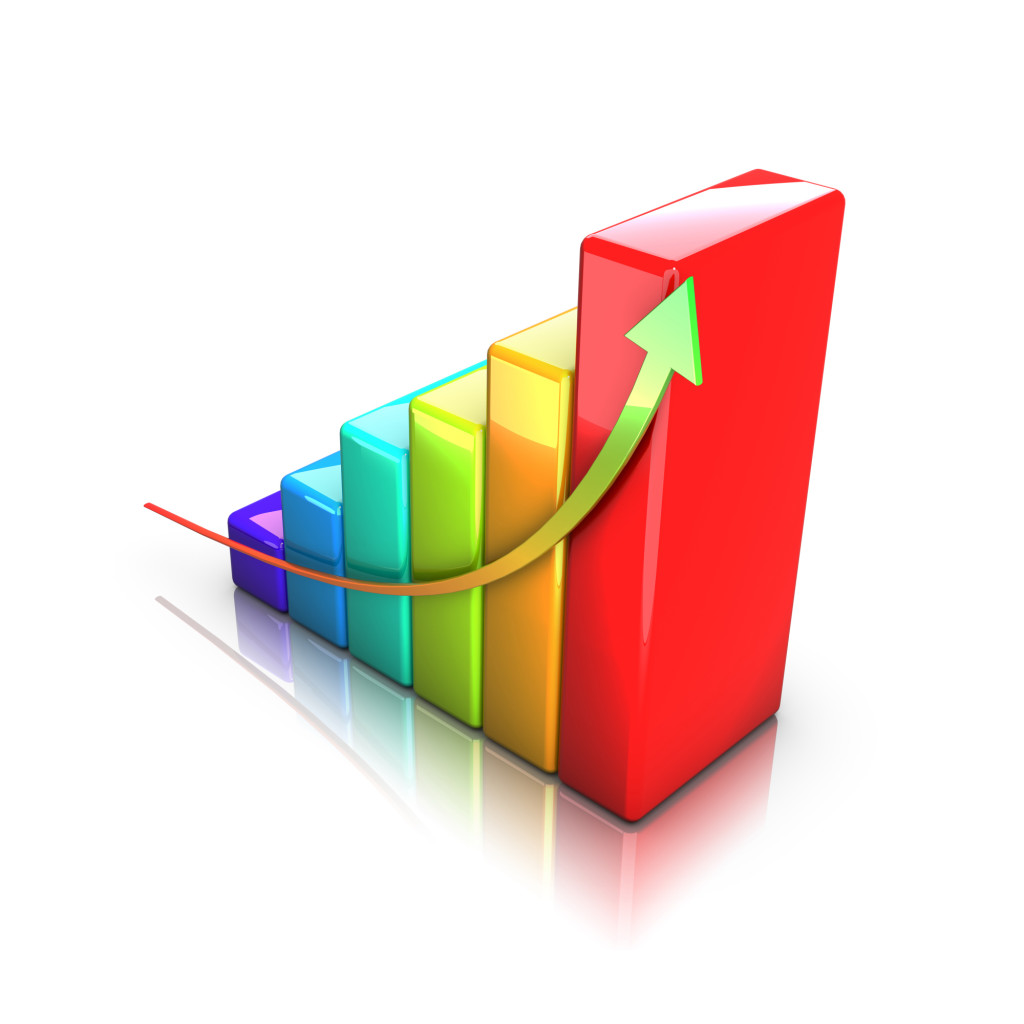
\includegraphics[width=8cm]{graph1.jpg}
\caption{Simulation results}
\label{grafik1}
\end{center}
\end{figure}
%okruzenje za postavljanje slike
%u uglastim zagradama sugerišete gde biste voleli da se slika prikaže, takozvani "float"
%[t] bi stavilo sliku na vrh strane, a [b] na dno; [h] znači "here" tj ovde postavi sliku
%znak uzvika ! kaze "potrudi se više da sliku staviš ranije"
%kombinovanjem komandi dajete programu veću slobodu da izabere gde da stavi sliku, ekstreman
%primer je [hbtp]
% Note that IEEE typically puts floats only at the top, even when this
% results in a large percentage of a column being occupied by floats.
% Note that IEEE does not put floats in the very first column - or typically
% anywhere on the first page for that matter. Also, in-text middle ("here")
% positioning is not used. Most IEEE journals/conferences use top floats
% exclusively. 

The learner was a confederate who would pretend to be shocked. As the experiment progressed, 
the teacher would hear the learner plead to be released and complain about a heart condition. 
Once the 300-volt level had been reached, the learner banged on the wall and demanded to be 
released. Beyond this point, the learner became completely silent and refused to answer any 
more questions. The experimenter then instructed the participant to treat this silence as an 
incorrect response and deliver a further shock. \cite{francis1993volcanoes}

When asking the experimenter if they should stop, they were instructed to continue. \cite{milgram1978obedience}.


\section{Results}
\label{sec_results}

Of the 40 participants in the study, 26 delivered the maximum shocks. 14 persons 
did not obey the experimenter and stopped before reaching the highest levels. All 40 
participants continued to give shocks up to 300 volts. Break-down of shocks given
has been provided in Table \ref{tbl_voltages}

\begin{table}[h]
\centering
\begin{tabular}{ l | c | r }
  Name & Voltage & Give up \\
  \hline %nova horizontalna linija
  John Doe & 300 & 98\% \\ %pošto je procenat poseban znak, pre njega se stavlja kosa crta da bi se prikazao bez interpretacije LaTeXa
  Jane Doe & 250 & Yes \\
  Some Guy & 300 & Yes\\
\end{tabular}
  \caption{Voltage reached}
  \label{tbl_voltages}
\end{table}
% An example of a floating table. Note that, for IEEE style tables, the 
% \caption command should come BEFORE the table. Table text will default to
% \footnotesize as IEEE normally uses this smaller font for tables.
% The \label must come after \caption as always.

\lipsum [1-3] %još malo nasumičnog teksta. Pogledajte kako se ovaj tekst umetnuo delimično pre tabele I, da bi se popunila stranica.

Tabela \ref{tabela2} pokazuje još jedan primer tabele, koja je malo raširena, dok je naslov tabele iznad same tabele, što je uobičajeno.

% 
\begin{table}[!hbtp]
%% increase table row spacing, adjust to taste
\renewcommand{\arraystretch}{2.4}
\caption{Primer tabele}
\label{tabela2}
\centering
%% Some packages, such as MDW tools, offer better commands for making tables
%% than the plain LaTeX2e tabular which is used here.
\begin{tabular}{l|||c|r} %prva kolona je levo postavljena, druga centralno, treca desno (left, center, right)
%broj uspravnih linija govori o tome koliko će linija biti iscrtano u tabeli između kolona, probajte da ih izbrišete ili dodate
\hline
Grupa & Prosečno vreme & Uspešnost\\
\hline %nova horizontalna linija
1 & 45 sekundi & 98\%\\ %pošto je procenat poseban znak, pre njega se stavlja kosa crta da bi se prikazao
\hline
2 & 48 sekundi & 92\%\\ 
\hline
\end{tabular}
\end{table}

\lipsum [4-6]

Slika \ref{cicamaca} pokazuje kako postaviti široku sliku. %Pogledajte kako i ovde slika odmah sledi tekst, ali biva postavljena na početak sledeće strane, radi boljeg vizuelnog ugođaja

\begin{figure*}[!ht] 
\centering
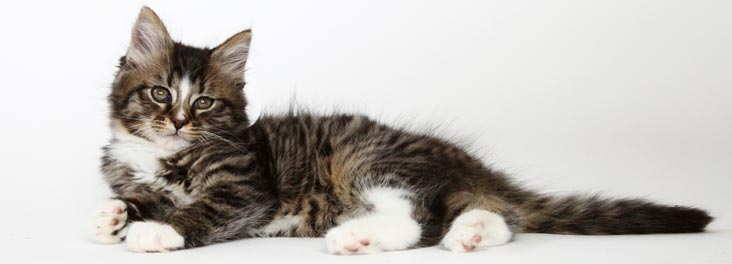
\includegraphics[width=0.95\textwidth]{graph2.jpg}
\caption{Primer široke slike koja treba da ide preko većeg dela stranice; da je forsiramo u jednu kolonu, bila bi suviše sitna}
\label{cicamaca}
\end{figure*}

%u ovom slučaju, slika zauzima 95% širine teksta na stranici
%zvezdice u {figure*} govore da se preskoči lokalno okruženje od dve kolone
%da izbrišete obe zvezdice i širinu promenite na "columnwidth", dobili biste sliku u jednoj koloni
%obratite pažnju kako su gornje dve slike ovde navedene jedna uz drugu, 
%ali ih LATEX ne postavlja blizu u PDFu

\lipsum [1-4]

\section{Discussion}
\label{sec_discussion}

Most of the participants became very agitated, stressed and angry at the experimenter \cite{vrgovic2012open}. 
Many continued to follow orders all the time even though they were clearly uncomfortable. 
The study shows that people are able to harm others intentionally if ordered to do so. It 
shows that the situation is far more important than previously believed, and that personal 
characteristics are less important in such a situation. \cite{frakes1992information}

\appendices
\section{Proof of the First Zonklar Equation}
Appendix one text goes here.

% you can choose not to have a title for an appendix
% if you want by leaving the argument blank
\section{}
Appendix two text goes here.



% use section* for acknowledgement
\section*{Dodatne napomene ili zahvalnica}
%pošto je ovo u okviru "appendices" dela, da nema zvezdice i ovaj deo bi bio označen kao prilog, npr "prilog C"
%zvezdica uvek relativizuje ili poništava lokalno okruženje


The authors would like to thank...


% references section

% can use a bibliography generated by BibTeX as a .bbl file
% BibTeX documentation can be easily obtained at:
% http://www.ctan.org/tex-archive/biblio/bibtex/contrib/doc/
% The IEEEtran BibTeX style support page is at:
% http://www.michaelshell.org/tex/ieeetran/bibtex/
\bibliographystyle{IEEEtran}
% argument is your BibTeX string definitions and bibliography database(s)
\bibliography{./reference}
%ovde se poziva na fajl u kom se reference nalaze, a to je fajl reference.bib
%otvorite .bib fajl pomoću bilo kog text editora da biste dodali ili izmenili reference
%na sajtu www.scholar.google.com pronađite rad koji vas zanima
%kliknite opciju "cite" pri dnu pojedinačnog rezultata
%kliknite opciju "BibTeX" pri dnu
%iskopirajte dobijeni tekst u vaš .bib fajl
%obratite pažnju na ključnu reč tog rada, nalazi se u prvoj liniji zapisa, desno od vitičaste zagrade
%na primer @article{pawlak1981information,
%citirajte rad u ovom .tex fajlu tako što pišete \cite{pawlak1981information}
%
%
%VAŽNO!!!!!!!!!!!!!!!!!!!!!!!!!!!!!!!!!
%da bi se rad uveo u sistem, u opciji "Quick build", koju vidite iznad, izaberite opciju "BibTeX" iz padajućeg menija
%kliknite strelicu pored Quick Build tako da uradite Run 
%iz padajućeg menija sada vratite na opciju "Quick build"
%i buildujte opet rad bar dva puta. Nakon ovoga trebalo bi da se pojavi referenca na svim mestima.


% that's all folks
\end{document}